\documentclass{article}
\usepackage{graphicx}
\usepackage[margin=1.5cm]{geometry}
\usepackage{amsmath}

\begin{document}
\twocolumn

\title{Wednesday Warm Up: Unit 0: Electrostatics I and II}
\author{Prof. Jordan C. Hanson}

\maketitle

\section{Memory Bank}

\begin{itemize}
\item 1\textit{e} = $1.602 \times 10^{-19}$ C ... Fundamental unit of charge.
\item $\vec{E} = \frac{k Q}{r^2} \hat{r}$ ... Coulomb field of a charge $Q$.
\item $k = 8.988 \times 10^{9}$ N C$^{-2}$ m$^{2}$ ... Constant of proportionality for Coulomb field.
\item $\vec{F} = q\vec{E}$ ... The force on a charge $q$ by a field $\vec{E}$.
\end{itemize}
\normalsize

\section{Electric Fields}

\begin{enumerate}
\item Consider Fig. \ref{fig:ring} below.  A ring of charge with radius $R$ is situated in the xy-plane.  The charge is positive, and it is distributed evenly across the ring.  We write $\Delta q = \lambda R \Delta\theta$, to mean that there are $\lambda$ Coulombs per meter along an angle $\Delta \theta$.  If $\Delta\theta$ were to extend to $2\pi$ (all the way around the circle), then the total charge is $Q = \lambda (2 \pi R)$.  (a) By \textit{symmetry}, where should the electric field be zero?  (b) Where would the electric field be infinite?
\begin{figure}[ht]
\centering
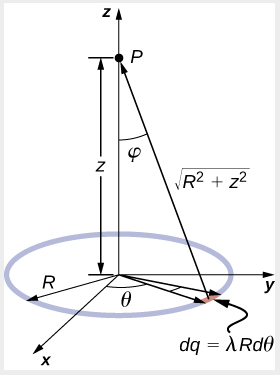
\includegraphics[width=0.22\textwidth]{figures/ring.png}
\caption{\label{fig:ring} A ring of charge situated in the xy-plane.}
\end{figure}
\item Consider again Fig. \ref{fig:ring}.  As $z \rightarrow \infty$, what happens to the field?
\begin{itemize}
\item A: The field-strength increases.
\item B: The field-strength remains constant.
\item C: The field-strength decreases.
\item D: The field-strength is exactly zero.
\end{itemize}
\item Suppose the actual function for the E-field $\vec{E}(z)$ is
\begin{equation}
\vec{E}(z) = \frac{k Q z}{\left( z^2 + R^2 \right)^{3/2}} \hat{z} \label{eq:eq1}
\end{equation}
To see what happens when $z$ is much larger than $R$, try setting $R=0$.  What is the result in Eq. \ref{eq:eq1} if $R=0$? \\ \vspace{1cm}
\item Do you recognize the expression?  What does the ring resemble if $R \approx 0$? \\ \vspace{3cm}
\item Suppose a test-charge $q = 1$ nC is placed at $z = 20$ cm above a ring of radius $R = 2$ cm. (a) What is the value $\vec{E}$, in N C$^{-1}$? (b) What is the force on $q$? (c) How many units of charge constitute $q$?
\end{enumerate}


\end{document}
